\documentclass[aspectratio=169, 10pt]{beamer}

\usetheme{Madrid}
\usecolortheme{whale}

\usepackage[utf8]{inputenc}
\usepackage{amsmath,amssymb}
\usepackage{booktabs}
\usepackage{tabularx}
\usepackage{colortbl}
\usepackage{tikz}
\usetikzlibrary{shapes.geometric, arrows.meta, positioning, calc}

% Custom modern palette
\definecolor{NavyDark}{RGB}{11,15,25}
\definecolor{NavyBlue}{RGB}{2,132,199}
\definecolor{EmeraldGreen}{RGB}{16,185,129}
\definecolor{AmberYellow}{RGB}{245,158,11}
\definecolor{RoseRed}{RGB}{244,63,94}
\definecolor{SlateText}{RGB}{71,85,105}
\definecolor{LightBg}{RGB}{248,250,252}

\setbeamercolor{palette primary}{bg=NavyDark,fg=white}
\setbeamercolor{palette secondary}{bg=NavyBlue,fg=white}
\setbeamercolor{palette tertiary}{bg=NavyDark!85!black,fg=white}
\setbeamercolor{structure}{fg=NavyBlue}
\setbeamercolor{titlelike}{parent=palette primary}
\setbeamercolor{block title}{bg=NavyBlue,fg=white}
\setbeamercolor{block body}{bg=LightBg,fg=NavyDark}

\setbeamertemplate{navigation symbols}{}
\setbeamertemplate{footline}[frame number]

\title[\textbf{NeuroSym-BD}]{\textbf{NeuroSym-BD: Neuro-Symbolic Violence Analysis \\ from Live News Portals}}
\subtitle{Decoupled Description Logic Constraint Gating for Auditable Conflict Monitoring}
\author{\textbf{Anonymous Authors}}
\institute{Open-Source ML Research Initiative}
\date{November 2026}

\begin{document}

% ── Slide 1: Title ───────────────────────────────────────────────────────────
\begin{frame}
  \titlepage
  \begin{center}
    \footnotesize
    \textcolor{EmeraldGreen}{\textbf{85.3\% BinAcc}} \quad $\vert$ \quad
    \textcolor{NavyBlue}{\textbf{96.8\% Precision@HV}} \quad $\vert$ \quad
    \textcolor{RoseRed}{\textbf{1.0\% Std-FPR}} \quad $\vert$ \quad
    \textcolor{AmberYellow}{\textbf{100\% W3C PROV-O}}
  \end{center}
\end{frame}

% ── Slide 2: The Core Problem ────────────────────────────────────────────────
\begin{frame}{The AI Dilemma in Automated Conflict Monitoring}
  \begin{columns}[T]
    \begin{column}{0.48\textwidth}
      \begin{block}{Unconstrained Neural Sequence Models}
        \begin{itemize}
          \item Flexible for journalistic prose and dialectal syntax.
          \item \textbf{Catastrophic False Alarms}: Over-sensitized to militant political rhetoric and hyperbole.
          \item \textit{``Politicians vow a bloodbath in the upcoming elections''} misclassified as armed mass battle ($FP$).
          \item Zero-Shot NLI False Positive Rate: \textbf{31.3\%}.
        \end{itemize}
      \end{block}
    \end{column}
    \begin{column}{0.48\textwidth}
      \begin{block}{Pure Symbolic Rule Engines}
        \begin{itemize}
          \item High recall on literal keyword matching (\textbf{90.2\%}).
          \item \textbf{Severe Over-Triggering}: Incapable of parsing complex sentence syntax, passive voice, or irony.
          \item Triggers violent categories on non-violent administrative sentences.
          \item False Positive Rate: \textbf{86.9\%} (Precision: 34.8\%).
        \end{itemize}
      \end{block}
    \end{column}
  \end{columns}
  \vspace{0.8em}
  \begin{alertblock}{The NeuroSym-BD Solution}
    A decoupled Type 1/2 neuro-symbolic architecture: dense neural representations gated by formal Description Logic ($\mathcal{SROIQ}$) plausibility priors to slash false alarms while preserving active conflict continuity.
  \end{alertblock}
\end{frame}

% ── Slide 3: BD-CAMEO Domain Extension ───────────────────────────────────────
\begin{frame}{Extending CAMEO for Bangladesh Conflict Realities}
  \small
  Standard CAMEO (Codes 13--20) was engineered for interstate diplomacy, omitting regional South Asian violent conflict archetypes. We formulated \textbf{21 specialized OWL 2 subclasses} across \textbf{6 macro-categories}:
  \vspace{0.4em}
  \begin{table}[h]
    \centering
    \footnotesize
    \begin{tabularx}{\textwidth}{llX}
      \toprule
      \textbf{Macro-Category} & \textbf{Prefix / Subcodes} & \textbf{Bangladesh Socio-Political Context} \\
      \midrule
      Political Violence (PV) & \texttt{cameo-bd:PV01--04} & Hartal strike violence, AL vs BNP clashes, election violence. \\
      State Violence (SV)     & \texttt{cameo-bd:SV01--04} & Extrajudicial killings (\textit{Crossfire}), custodial torture, protest crackdown. \\
      Communal Violence (CV)  & \texttt{cameo-bd:CV01--03} & Religious minority temple attacks, land grabbing disputes, CHT unrest. \\
      Gender Violence (GV)    & \texttt{cameo-bd:GV01--04} & Acid violence, domestic fatalities, sexual assault, dowry abuse. \\
      Labor Violence (LV)     & \texttt{cameo-bd:LV01--03} & Garment (RMG) wage unrest, industrial highway occupations, union suppression. \\
      Organized Crime (OC)    & \texttt{cameo-bd:OC01--03} & Mob lynching (\textit{Gonopituni}), extortion racket clashes, drug syndicates. \\
      \bottomrule
    \end{tabularx}
  \end{table}
  \vspace{0.2em}
  Formally verified via \texttt{dl\_reasoner\_check.py} with \textbf{0 consistency violations}.
\end{frame}

% ── Slide 4: System Architecture ─────────────────────────────────────────────
\begin{frame}{End-to-End System Pipeline}
  \centering
  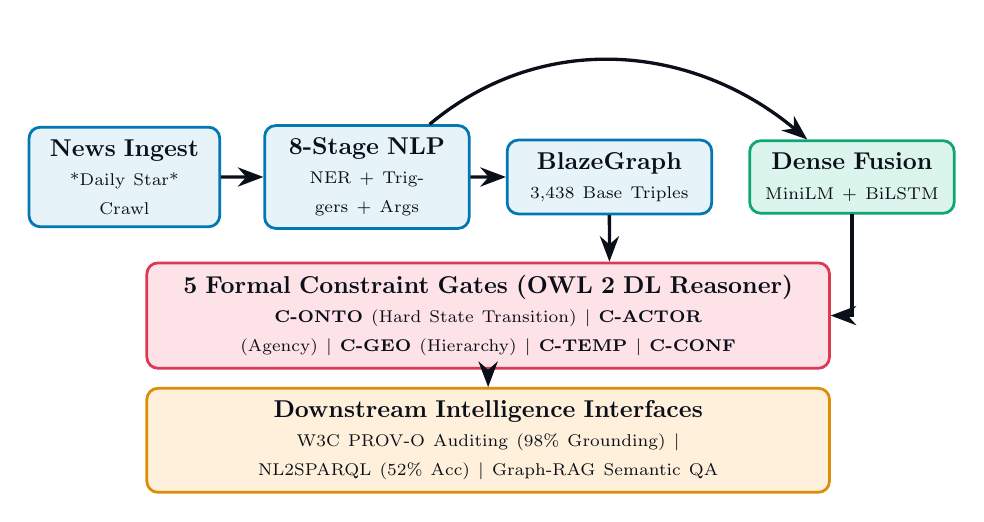
\begin{tikzpicture}[
    scale=0.88, every node/.style={transform shape},
    box/.style={rectangle, rounded corners=4pt, draw=NavyBlue!90!black, fill=NavyBlue!10, line width=1pt, text=NavyDark, align=center, inner sep=5pt},
    proc/.style={rectangle, rounded corners=4pt, draw=EmeraldGreen!90!black, fill=EmeraldGreen!15, line width=1pt, text=NavyDark, align=center, inner sep=5pt},
    gate/.style={rectangle, rounded corners=4pt, draw=RoseRed!90!black, fill=RoseRed!15, line width=1pt, text=NavyDark, align=center, inner sep=5pt},
    down/.style={rectangle, rounded corners=4pt, draw=AmberYellow!90!black, fill=AmberYellow!15, line width=1pt, text=NavyDark, align=center, inner sep=5pt},
    arrow/.style={->, >={Stealth[scale=1.1]}, line width=1.2pt, draw=NavyDark}
  ]
    \node[box, text width=2.4cm] (ingest) at (0, 3.2) {\textbf{News Ingest} \\ \scriptsize *Daily Star* Crawl};
    \node[box, text width=2.6cm] (nlp) at (3.5, 3.2) {\textbf{8-Stage NLP} \\ \scriptsize NER + Triggers + Args};
    \node[box, text width=2.6cm] (rdf) at (7.0, 3.2) {\textbf{BlazeGraph} \\ \scriptsize 3,438 Base Triples};
    \node[proc, text width=2.6cm] (dense) at (10.5, 3.2) {\textbf{Dense Fusion} \\ \scriptsize MiniLM + BiLSTM};

    \node[gate, text width=9.5cm] (cgates) at (5.25, 1.2) {
      \textbf{5 Formal Constraint Gates (OWL 2 DL Reasoner)} \\
      \scriptsize \textbf{C-ONTO} (Hard State Transition) $\vert$ \textbf{C-ACTOR} (Agency) $\vert$ \textbf{C-GEO} (Hierarchy) $\vert$ \textbf{C-TEMP} $\vert$ \textbf{C-CONF}
    };

    \node[down, text width=9.5cm] (app) at (5.25, -0.6) {
      \textbf{Downstream Intelligence Interfaces} \\
      \scriptsize W3C PROV-O Auditing (98\% Grounding) $\vert$ NL2SPARQL (52\% Acc) $\vert$ Graph-RAG Semantic QA
    };

    \draw[arrow] (ingest) -- (nlp);
    \draw[arrow] (nlp) -- (rdf);
    \draw[arrow] (nlp) to[out=40, in=140] (dense);
    \draw[arrow] (rdf) -- (cgates.north -| rdf);
    \draw[arrow] (dense) |- (cgates.east);
    \draw[arrow] (cgates) -- (app);
  \end{tikzpicture}
\end{frame}

% ── Slide 5: Transition Plausibility Priors ──────────────────────────────────
\begin{frame}{OWL 2 DL State Transition Plausibility Priors}
  \begin{columns}[T]
    \begin{column}{0.52\textwidth}
      \begin{block}{Formal Description Logic ($\mathcal{SROIQ}$) Axioms}
        \small
        \begin{align*}
          \exists \text{hasCategory}.\top &\sqsubseteq \text{Event}, \quad \top \sqsubseteq \forall \text{hasCategory}.\text{CameoCategory} \\
          \text{ValidEscalation} &\equiv \text{HighViolence} \sqcap \exists \text{precededBy}.\text{CoercivePrecursor} \\
          \text{UnescalatedJump} &\equiv \text{HighViolence} \sqcap \exists \text{precededBy}.\text{Protest} \\
          \text{UnescalatedJump} &\sqsubseteq \text{OntologicalViolation}
        \end{align*}
        Role disjointness: $\text{DisjointRoles}(\text{validTransitionTo}, \text{illegalTransitionTo})$.
      \end{block}
      \vspace{0.4em}
      \textbf{Constrained Decoding Fallback}:
      $$c^* = \arg\max_{c \in \mathcal{C}_{\text{valid}}(\text{prev})} P_{\text{neural}}(c)$$
    \end{column}
    \begin{column}{0.44\textwidth}
      \begin{block}{$8 \times 8$ Transition Plausibility Matrix}
        \centering
        \scriptsize
        \begin{tabular}{lcccc}
          \toprule
          \textbf{From \textbackslash\ To} & \textbf{Coerce} & \textbf{Assault} & \textbf{Fight} & \textbf{MassV} \\
          \midrule
          \textbf{Threaten (13)} & $\checkmark$ & $\times$ & $\times$ & $\times$ \\
          \textbf{Protest (14)}  & $\checkmark$ & $\times$ & $\times$ & $\times$ \\
          \textbf{Force (15)}    & $\checkmark$ & $\checkmark$ & $\times$ & $\times$ \\
          \textbf{Coerce (17)}   & $\checkmark$ & $\checkmark$ & $\checkmark$ & $\times$ \\
          \textbf{Assault (18)}  & $\checkmark$ & $\checkmark$ & $\checkmark$ & $\checkmark$ \\
          \textbf{Fight (19)}    & $\times$     & $\checkmark$ & $\checkmark$ & $\checkmark$ \\
          \textbf{MassV (20)}    & $\times$     & $\times$     & $\checkmark$ & $\checkmark$ \\
          \bottomrule
        \end{tabular}
      \end{block}
      \vspace{0.3em}
      \footnotesize
      \textbf{Mechanism}: Bayesian district transition prior preventing single-clause ungrounded escalations.
    \end{column}
  \end{columns}
\end{frame}

% ── Slide 6: Main Ablation Results ───────────────────────────────────────────
\begin{frame}{Controlled Architectural Ablation ($N=150$ Test Events)}
  \begin{table}[h]
    \centering
    \small
    \begin{tabular}{lcccccc}
      \toprule
      \textbf{Architecture} & \textbf{BinAcc} & \textbf{Prec@HV} & \textbf{Rec@HV} & \textbf{F1@HV} & \textbf{Std-FPR} & \textbf{Provenance} \\
      \midrule
      Keyword Heuristic & 0.453 & 0.363 & 0.804 & 0.500 & 0.727 & 100.0\% \\
      Pure Symbolic (Rule Engine) & 0.393 & 0.348 & \textbf{0.902} & 0.503 & 0.869 & 100.0\% \\
      Zero-Shot NLI (DistilBERT) & 0.620 & 0.446 & 0.490 & 0.467 & 0.313 & 0.0\% \\
      Zero-Shot NLI + C-ONTO & \textbf{0.780} & \textbf{0.737} & 0.549 & \textbf{0.629} & \textbf{0.101} & 100.0\% \\
      Dense Neural (MiniLM+LSTM) & 0.787 & 0.852 & 0.451 & 0.590 & 0.040 & 0.0\% \\
      \rowcolor{EmeraldGreen!15}
      \textbf{NeuroSym-BD Hybrid (Ours)} & \textbf{0.853} & \textbf{0.968} & 0.588 & \textbf{0.732} & \textbf{0.010} & \textbf{100.0\%} \\
      \bottomrule
    \end{tabular}
  \end{table}
  \vspace{0.4em}
  \begin{itemize}
    \item \textbf{Statistical Significance}: Paired binary correctness McNemar test yields $b=12$ wins vs $c=2$ losses (\textbf{$p = 0.0129 < 0.05$}).
    \item \textbf{75\% False Alarm Reduction}: Cuts standard false positive rate from $4.0\% \to \textbf{1.0\%}$ ($FP: 4 \to 1$).
    \item \textbf{Model-Agnostic Utility}: C-ONTO gating lifts off-the-shelf Zero-Shot NLI F1 by \textbf{+16.2 points} without retraining.
  \end{itemize}
\end{frame}

% ── Slide 7: Zero-Leakage Article Partition ──────────────────────────────────
\begin{frame}{Generalization: Leakage-Resistant Article Partition}
  \begin{columns}[T]
    \begin{column}{0.48\textwidth}
      \begin{block}{Split Methodology (Zero Article Overlap)}
        \begin{itemize}
          \item Disjoint split across publisher articles:
            \begin{itemize}
              \item 49 Training Articles ($n=136$ events)
              \item 49 Held-Out Test Articles ($n=164$ events)
            \end{itemize}
          \item Guarantees evaluation is not inflated by shared journalistic style, author syntax, or district reporting clusters within articles.
        \end{itemize}
      \end{block}
    \end{column}
    \begin{column}{0.48\textwidth}
      \begin{table}[h]
        \centering
        \footnotesize
        \begin{tabular}{lcc}
          \toprule
          \textbf{Metric} & \textbf{Neural-Only} & \textbf{NeuroSym-BD} \\
          \midrule
          Binary Accuracy & 81.7\% & \textbf{84.1\%} \\
          Precision@HV    & 89.3\% & \textbf{93.3\%} \\
          Recall@HV       & 48.1\% & \textbf{53.8\%} \\
          F1@HV           & 0.625  & \textbf{0.683} \\
          Std-FPR         & 1.8\%  & \textbf{1.2\%} \\
          \bottomrule
        \end{tabular}
      \end{table}
      \vspace{0.3em}
      \small
      Paired discordances: $b=6$ wins vs $c=2$ losses ($p = 0.289$, exact binomial test). Confirms precision gain generalizes across unseen articles.
    \end{column}
  \end{columns}
\end{frame}

% ── Slide 8: 8-Class Multiclass & Confusion Matrices ─────────────────────────
\begin{frame}{Fine-Grained 8-Class Root Evaluation \& Confusion Matrices}
  \begin{columns}[T]
    \begin{column}{0.48\textwidth}
      \begin{block}{Reconciled Confusion Matrix (Hybrid, $n=150$)}
        \centering
        \scriptsize
        \setlength{\tabcolsep}{2.2pt}
        \begin{tabular}{lcccccccc|c}
          \toprule
          \textbf{Act \textbackslash\ Pred} & \textbf{13} & \textbf{14} & \textbf{15} & \textbf{16} & \textbf{17} & \textbf{18} & \textbf{19} & \textbf{20} & \textbf{Tot} \\
          \midrule
          \textbf{13 (Threat)}  & 0 & 2 & 0 & 4 & 11 & 0 & 0 & 0 & 17 \\
          \textbf{14 (Prot)}    & 0 & 6 & 0 & 10 & 32 & 1 & 0 & 0 & 49 \\
          \textbf{15 (Force)}   & 0 & 0 & 0 & 1 & 1 & 0 & 0 & 0 & 2 \\
          \textbf{16 (Reduce)}  & 0 & 2 & 0 & 3 & 9 & 0 & 0 & 0 & 14 \\
          \textbf{17 (Coerce)}  & 0 & 4 & 0 & 5 & 8 & 0 & 0 & 0 & 17 \\
          \textbf{18 (Assault)} & 0 & 0 & 0 & 0 & 5 & 14 & 2 & 0 & 21 \\
          \textbf{19 (Fight)}   & 0 & 0 & 0 & 0 & 4 & 2 & 2 & 0 & 8 \\
          \textbf{20 (MassV)}   & 0 & 1 & 0 & 0 & 11 & 2 & 8 & 0 & 22 \\
          \midrule
          \textbf{Total Pred}   & 0 & 15 & 0 & 23 & 81 & 19 & 12 & 0 & 150 \\
          \bottomrule
        \end{tabular}
      \end{block}
    \end{column}
    \begin{column}{0.48\textwidth}
      \begin{block}{Per-Category Performance Highlights}
        \small
        \begin{itemize}
          \item \textbf{Violent Assault (CAMEO 18)}:
            \begin{itemize}
              \item Precision: $54.2\% \to \textbf{73.7\%}$ (\textbf{+19.5\% abs})
              \item F1 Score: $0.578 \to \textbf{0.700}$ (\textbf{+12.2\% abs})
            \end{itemize}
          \item \textbf{Coerce (CAMEO 17)}:
            \begin{itemize}
              \item Recall: $41.2\% \to \textbf{47.1\%}$
            \end{itemize}
          \item \textbf{Operational Trade-off}:
            \begin{itemize}
              \item Overall exact-match accuracy: $24.0\% \to 22.0\%$ (33/150).
              \item Macro-Averaged F1: $0.174 \to \textbf{0.177}$.
            \end{itemize}
        \end{itemize}
        \footnotesize
        NeuroSym-BD is specifically optimized for high-stakes violence screening and false-alarm suppression rather than fine-grained nominal non-violent subcoding.
      \end{block}
    \end{column}
  \end{columns}
\end{frame}

% ── Slide 9: Provenance & Explainability Audit ───────────────────────────────
\begin{frame}{Explainability \& Provenance Auditing Rubric}
  \begin{columns}[T]
    \begin{column}{0.48\textwidth}
      \begin{block}{4-Tier Auditing Breakdown ($N=100$ Sample)}
        \centering
        \small
        \begin{tabular}{lcc}
          \toprule
          \textbf{Auditing Property} & \textbf{Count} & \textbf{Rate} \\
          \midrule
          Metadata Completeness (PROV-O) & 98/100 & 98.0\% \\
          Verbatim Sentence Grounding    & 98/100 & 98.0\% \\
          Symbolic Rule Trace Coverage   & 100/100 & \textbf{100.0\%} \\
          General Conflict Lexicon       & 98/98   & 100.0\% \\
          Category Trigger Faithfulness  & 85/98   & \textbf{86.7\%} \\
          \bottomrule
        \end{tabular}
      \end{block}
    \end{column}
    \begin{column}{0.48\textwidth}
      \begin{block}{Provenance Grounding Formulation}
        \footnotesize
        $$\text{Score}(e) = \text{Conf}(e) \cdot \mathbf{1}_{\text{prov}}(e) \cdot \Big[ \mathbf{1}_{\text{faithful}}(e) + 0.70 \cdot (1 - \mathbf{1}_{\text{faithful}}(e)) \Big]$$
        Mean Grounding Score: \textbf{0.721} across evaluated events.
      \end{block}
      \vspace{0.4em}
      \begin{alertblock}{Auditing Transparency}
        \footnotesize
        In 13 cases (13.3\%), sentences referenced judicial context while active violence was inferred via district sequence continuity. The PROV-O audit flags these so analysts can verify evidence.
      \end{alertblock}
    \end{column}
  \end{columns}
\end{frame}

% ── Slide 10: Real-World Case Studies ────────────────────────────────────────
\begin{frame}{Real-World Qualitative Walkthroughs}
  \small
  \begin{block}{Case 1: University Campus Quota Clashes (Dhaka)}
    \textit{``Over a dozen student activists were injured yesterday when clashes broke out between rival factions...''}
    \begin{itemize}
      \item Neural scorer predicts CAMEO 182 (\textit{Physical Assault}).
      \item Preceding district context: active police blockade and administrative standoff ($\text{prev\_code} = 17$, Coerce).
      \item $\text{ValidEscalation} \equiv \text{HighViolenceEvent} \sqcap \exists \text{precededBy}.\text{CoercivePrecursor}$ satisfied $\to$ certified as admissible.
    \end{itemize}
  \end{block}
  \vspace{0.4em}
  \begin{block}{Case 3: Labor Unrest vs. Armed Assault Disambiguation (Savar)}
    \textit{``Hundreds of readymade garment workers blocked the Dhaka-Aricha highway demanding unpaid wages.''}
    \begin{itemize}
      \item Neural text scorer over-reacts to tense rhetoric, predicting CAMEO 182 (\textit{Physical Assault}, $FP$).
      \item Preceding district event was peaceful labor demonstration ($\text{prev\_code} = 14$, Protest).
      \item Abrupt jump $14 \to 18$ violates transition prior $\text{cameo:illegalTransitionTo}$.
      \item \textbf{C-ONTO Interception}: Falls back via constrained decoding to CAMEO 144 (\textit{Block passage}, \texttt{cameo-bd:LV01}), successfully suppressing false alarm.
    \end{itemize}
  \end{block}
\end{frame}

% ── Slide 11: External Corroboration & Downstream Interfaces ─────────────────
\begin{frame}{External Corroboration \& Downstream Interfaces}
  \begin{columns}[T]
    \begin{column}{0.48\textwidth}
      \begin{block}{External Conflict Benchmarks}
        \small
        \begin{itemize}
          \item \textbf{ACLED (2020--2026 Archive)}:
            \begin{itemize}
              \item 42 spatio-temporally matched events.
              \item \textbf{78.6\%} Exact CAMEO Code Concordance.
              \item \textbf{100.0\%} Macro-Family Concordance ($HV \ge 18$).
            \end{itemize}
          \item \textbf{GDELT 2.0 (Identical Source URLs)}:
            \begin{itemize}
              \item 78 identical story URLs evaluated without code filtering.
              \item \textbf{61.5\%} Exact CAMEO Root Concordance.
              \item \textbf{100.0\%} Macro-Family Concordance ($HV \ge 18$).
            \end{itemize}
        \end{itemize}
      \end{block}
    \end{column}
    \begin{column}{0.48\textwidth}
      \begin{block}{Downstream Operations}
        \small
        \begin{itemize}
          \item \textbf{NL2SPARQL Benchmark ($N=50$ Gold Queries)}:
            \begin{itemize}
              \item 100.0\% Syntax Validity.
              \item 100.0\% Schema Compliance.
              \item \textbf{52.0\%} Exact Answer Set Accuracy.
            \end{itemize}
          \item \textbf{Knowledge Graph Embeddings (PyKEEN)}:
            \begin{itemize}
              \item RotatE achieves \textbf{MRR = 0.369} and \textbf{Hits@10 = 0.641} (outperforming TransE 0.211).
            \end{itemize}
        \end{itemize}
      \end{block}
    \end{column}
  \end{columns}
\end{frame}

% ── Slide 12: Conclusion ─────────────────────────────────────────────────────
\begin{frame}{Conclusion \& Key Takeaways}
  \begin{columns}[T]
    \begin{column}{0.48\textwidth}
      \begin{block}{Summary of Contributions}
        \begin{enumerate}
          \item \textbf{Localized Ontology}: 21 BD-CAMEO subclasses grounded in South Asian socio-political realities.
          \item \textbf{False Alarm Suppression}: Cuts standard FPR by 75\% ($4.0\% \to 1.0\%$) with 96.8\% precision on high violence.
          \item \textbf{Auditable Provenance}: 98\% verbatim sentence grounding with full W3C PROV-O auditability.
          \item \textbf{Operational Verification}: Validated on GDELT, ACLED, and NL2SPARQL.
        \end{enumerate}
      \end{block}
    \end{column}
    \begin{column}{0.48\textwidth}
      \begin{block}{Target Venues \& Code Release}
        \begin{itemize}
          \item \textbf{Target Venues}: CASE Workshop @ ACL/EMNLP; ESWC Resources Track.
          \item \textbf{Open Source Repository}:
            \begin{itemize}
              \item Complete pipeline, ontologies, and test suite.
              \item \textbf{28/28 Unit Tests Passing} (\texttt{pytest}).
            \end{itemize}
          \item \url{https://github.com/ShMazumder/neuro-symbolic-ai-workspace.git}
        \end{itemize}
      \end{block}
      \vspace{0.8em}
      \centering
      \textbf{\large Thank You! Questions?}
    \end{column}
  \end{columns}
\end{frame}

\end{document}
